
\documentclass[british,10pt,a4paper]{article}
\usepackage[british]{babel}
\usepackage[margin=1in, bottom=0.75in, top=0.75in, footskip=0.25in]{geometry}
\usepackage[titletoc]{appendix}
\usepackage{fancyhdr}
\usepackage{mathtools}
\usepackage[numbers]{natbib}
\usepackage{pgfplotstable,filecontents}
\usepackage{hyperref}
\usepackage{booktabs}
\usepackage{wrapfig}
\usepackage{listings}
\usepackage{color}
\usepackage{graphicx}
\usepackage{siunitx}
\usepackage[parfill]{parskip}
\usepackage{tikz} % To generate the plot from csv
\usepackage{pgfplots}
\usepgfplotslibrary{statistics}

\pgfplotsset{compat=newest} % Allows to place the legend below plot
\usepgfplotslibrary{units} % Allows to enter the units nicely

\graphicspath{ {images/} }

\setcounter{secnumdepth}{2}
\setcounter{tocdepth}{2}
\renewcommand{\arraystretch}{1.2}
\renewcommand\thesection{\arabic{section}}
\renewcommand\thesubsection{\roman{subsection}.}
\renewcommand\thesubsubsection{}
\newcommand*{\Appendixautorefname}{appendix}
\pagestyle{fancy}
\fancyhf{}
\renewcommand{\headrulewidth}{0pt}
\lfoot{Exam no: Y0076159}
\cfoot{\thepage}
\lstset{
  columns=fixed,
  breaklines=true,
  basicstyle=\ttfamily\footnotesize
  }

\usepackage[nottoc]{tocbibind}
\usepackage{csvsimple}

\begin{document}
\title{CTAP Open Assessment}
\author{Exam no: Y0076159}
\date{\today}
\maketitle
\tableofcontents
\clearpage
\section{Breaking Stream Ciphers}
\subsection{Implementation and Challenge}
The stream cipher implementation, found in \autoref{app:stream} (written in Python),
can be ran using the Python 2.7.6 compiler with the command \lstinline{python stream.py}. This will produce the
challenge 25 bit output of 3 Lfsrs with initial states 97, 975 and 6420:

1 0 1 0 1 0 1 1 1 0 1 0 1 1 0 0 0 0 0 0 1 0 0 1 1

\subsubsection{Code description}
The code found in \autoref{app:stream} implements the geffe cipher through the \lstinline{Lfsr} class, which implements an LFSR with a tap sequence, size and initial state. It contains 2 methods:
\lstinline{calc_tap()}, which calculates the tap value for the current register value, and \lstinline{shift} which
calculates the tap value, shifts the register and outputs the register's value. The 3 LFSR's are combined using
\lstinline{combine_lfsr_outputs}, which uses a lookup table to implement the boolean operation.

\subsection{Cryptanalysis}
\subsubsection{Analysis}

\begin{center}
	\begin{tabular}{lllp{6.5cm}}\label{tab:streamattack} \\
		\toprule \\
		Linear func.  & Walsh transform & Attack No & Attack description \\
		\midrule \\
		\(R_3\) & 0 \\
		\(R_2\) & 0 & & \\
		\(R_2 \oplus R_3\) & 0 & & \\
		\(R_1\) & -4 & 1 & No dependencies, has a single outlier agreement (see \autoref{app:lfsragreements}) \\
		\(R_1 \oplus R_3\) & -4 & 3 & Requires \(R_1\), attack with \(R_1 \oplus R_3 \oplus K\) \\
		\(R_1 \oplus R_2\) & 4 & 2 & Requires \(R_1\), attack with \(R_1 \oplus R_2 \oplus K\)\\
		\(R_1 \oplus R_2 \oplus R_3\) & -4 & & \\

		\bottomrule \\
	\end{tabular}
\end{center}
Using the Walsh transform displayed in \autoref{app:walsh}, we can implement a divide-and-conquer strategy as first detailed by \citet{siegenthaler}.
LFSR1 correlates quite strongly with the output (Walsh value of -4, 2 agreements and 6 disagreements resulting in a probability of 2/8 that it will agree with the function's output, with a bias of 0.25); this is reflected by the outlying value in the graph of sub-keys and their agreements with outputs in \autoref{app:lfsragreements}. As such, it can be brute-forced to obtain it's key value by iterating over the space of sub-keys, and finding the one with the highest agreement (sub-key value 27, with an agreement of 0.253).

It is not feasible to brute-force \(R_2\) due to a lack of correlation with the output, as demonstrated by the Walsh-Transform value of 0 and the lack of any outlying sub-key agreement (as visible in \autoref{app:lfsragreements}). The next attack targets \(R_1 \oplus R_2\), as it has a Walsh value of 4 (6 agreements and 2 disagreements resulting in a probability of 6/8, and a bias of -0.25). 
The search space is reduced from \(O(n^{7} * n^{11})=O(n^{18})\) to \(O(n^{11})\) as we now know the key for LFSR1, allowing us to rapidly brute force the sub key for LFSR2 (value 1357, with agreement 0.247).

Finally LFSR3 can be attacked using \(R_1 \oplus R_3\), with a Walsh value of -4 (same agreements, disagreements, probability of correlation and bias as the previous attack).
As LFSR1's key is known, the search space is also reduced for this attack from \(O(n^{7} * n^{13})=O(n^{20})\) to \(O(n^{13})\). This resulted in the sub-key for LFSR3 (value 7531, with agreement 0.245). This LFSR was also not brute-forcible due to a correlation with the output (as highlighted by the Walsh value of 0). This is also highlighted by the box-and-whisker plots in \autoref{app:lfsragreements}, where the biggest outlying agreement in LSFR3 is significantly closer to the median than the outlying agreement for LSFR1; this suggests a lower likelihood of the outlying key being correct.

Using this strategy, we have successfully attacked all 3 shift registers in a severely reduced search space (\(O(n^{7+11+13})>(O(n^{7}+n^{11}+n^{13})=O(n^{13}))\) (a reduction of 18 bits), resulting in the set of sub-keys: 27, 1357, and 7531.
\subsubsection{Attack Implementation}
The Python program (found in \autoref{app:streamattack}) implements this attack by first loading a keystream from \lstinline{block.txt}, and begins by brute forcing the first register.
This is achieved by iterating over all possible keys, recording their agreement with the given data, and returning the key with the highest normalized agreement.
The next 2 LFSR's are then broken by iterating over each respective set of possible keys in combination with the output of LFSR1 using the previously known key.
This results in the set of initial states: \lstinline{lfsr1: 27, lfsr2: 1357, lfsr3: 7531}.

\subsection{Improvement}
Within the context of correlation attacks, the current cipher's key weakness is the correlation of a single shift register (LFSR1) with the output: this allows the key to be brute forced in \(O(n^7)\), followed by the other two keys in \(O(n^{11})\) and \(O(n^{13})\).
As such, the current function is not correlation immune to any significant order, hence why it was significantly vulnerable to a divide and conquer attack. As demonstrated by \citet{siegenthaler}, improving this correlation immunity would greatly increase the complexity of a divide and conquer attack, as demonstrated below.

By changing the combination function's output to 1 0 0 1 0 1 1 0 (two bit flips on L001 and L101, found by manual experimentation), we can ensure the function
is correlation immune to order 2, as the Walsh-Hadamard values for \(R_1\),
\(R_2\),  \(R_3\),  \(R_1 \oplus R_2\), \(R_1 \oplus R_3\) and \(R_1 \oplus R_3\), are now 0,
and therefore have no exploitable correlation exist other than all 3 registers combined; this is visible in the table below.

\begin{center}
	\begin{tabular}{@{}lll@{}}\label{tab:walsh2} \\
		Input & \(f\) & \(w\) \\
		\midrule \\
		000   & 1     & 0     \\
		001   & 0     & 0     \\
		010   & 0     & 0     \\
		011   & 1     & 0     \\
		100   & 0     & 0     \\
		101   & 1     & 0     \\
		110   & 1     & 0     \\
		111   & 0     & -8    \\
		\bottomrule \\
	\end{tabular}
\end{center}
This would restrict the attack vector to a combination of LFSR1, LFSR2 and LFSR3 simultaneously, with a Walsh-Hadamard value of -8 for \(R_1 \oplus R_2 \oplus R_3\); this is acceptable as exploiting this would require iterating over the complete key-set \(O(n^{7+11+13}) = O(n^{31})\), causing the time complexity to be significantly higher than the previous \(O(n^{13}))\) (a maximal time complexity given the current keyspace). This would provide maximal resilience to a divide and conquer attack, but is extremely vulnerable to an algebraic attack, as discussed below.

\citet{courtois} details a newer form of attack on synchronous LFSR-based stream ciphers ("where each state is generated from the previous state independently of the plain-text") using a set of over-defined algebraic equations to approximate the output function, which allow him to greatly reduce the key-space; the case study used to detail his methodology involves breaking a single 128 bit LFSR cipher in \(2^{49}\) clock cycles. This vulnerability occurs due to a stream cipher's function using only a subset of state bits; this was novel for it's era as it showed a vulnerability in spite of satisfying all previously known security criteria. \citeauthor{courtois} adds to this criterion by stating that "there should be no non-trivial multivariate relations of low degree that relate key bits and one or many outputs bits of the cipher". Within the context of our Geffe generator, \citeauthor{courtois} would estimate a worst case time complexity of \(O(2.95 * 10^{11})\), a significant reduction compared to the \(O(n^{31})\) of our 'improved' boolean function. As such, a balance between resilience to divide \& conquer and algebraic attacks is necessary, and methods to generate functions resilient to both is an ongoing topic of research \cite{Carlet2010-ew}.

Measuring the robustness of a boolean function to algebraic attack was defined by \citet{Armknecht2006-sj}, whilst \citet{carlet} presented a methodology to generate boolean functions with maximum possible algebraic immunity, although the produced solutions had insufficient non-linearity, signifying a potential weakness to correlation attacks.


It would also be possible to add additional LSFR's to the cipher and adapting the boolean function to require all 4 LSFRs to be cracked simultaneously. In the same way that increasing the length of the registers, this would increase the complexity to \(O(n^{7+11+13+x})\) where \lstinline{x} is the length of the additional register, or the sum of the number of bits added to each LFSR.

These methods would provide resilience to a divide-and-conquer attack by increasing the order of correlation immunity, causing the key-space to remain as the product of the key-space sizes of each register rather than their sum. However, other forms of attacks on stream ciphers can make them vulnerable if the cipher is poorly designed. Keeping in mind that the previously suggested combination function may not be robust these cases, we will now explore various other attack methodologies on stream ciphers, and methods to improve the robustness of the cipher to these attacks.

The simplest of these is a reused key attack, where the same key is used to encrypt two different plain-texts; this constitutes a weakness in the usage of the cipher, rather than a statistical weakness. Using the commutative property of XOR, the two cipher texts can be XOR'd to cancel out the use of the random stream, and reveal \(A \oplus B\) (where A and B are plain-texts). If one of these message is known, retrieving the other's content is therefore trivial. This method was famously used to break the Lorenz cipher during WW2 \cite{sale}, but is easily fixable by using a pre-agreed method to generate one-time keys from a master key and initialisation vector. 

In addition, a bit-flipping attack is feasible which allows a man-in-the-middle attack or replay attack to vary the contents of a cipher-text without knowing it's key. This is feasible if the attacker knows part of the content of the cipher-text, as well as the location of the known content in the cipher-text. By XORing that section of the cipher text with his content, and XORing the result with the message which is being tampered. This results in a message which corresponds to what the sender would have sent using the information the attacker wished to insert into the message. This could be prevented by including a message authentication codes (MAC) such as the hash of the plain-text in the communication, which could then be used to verify whether the message was tampered without equivalent tampering of the MAC. This is detailed by \citet{Isaacs}, with a case study of vulnerabilities in the Wired Equivalent Privacy (WEP) algorithm for wireless networks.

An additional attack was demonstrated by \citet{helleseth}, who formulates a methodology based on using a minimal amount of key-stream bits. As such, to maximise a resistance to such an attack, increasing the cyclic period of the LFSRs would be necessary. This could be achieved by changing the tap function to one with a longer period, or extending the bit length of the register. A new class of boolean functions which are resistant to fast correlation attacks, Helleseth-Ronjom, Berlekamp-Massey and fast algebraic attacks was also presented by \citet{carlet2}.

Finally, \citet{massey} provided an adaptation of the Berklekamp algorithm which allows the estimation of the length of an LFSR given \citet{massey} given an upper-bounded number of bits of the output sequence. Given that this could reveal a hidden structure of the cipher, strengthening against this attack may be crucial. As previously stated, \citeauthor{carlet2} provides a boolean function generation which gives a good resistance to this attack in addition to others, whilst the more computationally expensive options of increasing the key-space through increased key-lengths and a larger number of LFSRs is also an alternative.

As such, suggested modifications to the cipher to improve it's robustness to common attacks would include lengthening the bit-width of each LFSR, adding LFSRs and utilising tap functions with maximal periods to increase the size of the key-space and resist Berlekamp-Massey attacks. The boolean combining function should be generated using \citeauthor{carlet2}\'s methodology \cite{carlet2}, (or alternately \citet{tang}) although given the pace at which this area of research continues to surpass itself it would not be surprising to find a better function generation methodology in the near future.

\clearpage
\section{Differential Cryptanalysis}
\subsection{Implementation and Challenge}
The block cipher found in \autoref{app:block} (written in Python),{}
can be ran using the Python 2.7.6 compiler with the command \lstinline{python block.py}. This will produce the
challenge output of 45858 (1011001100100010 in binary).
\subsection{Code description}
The full block cipher is implemented using the \lstinline{do_4_rounds()} method, which controls the execution of substitutions, permutations or combinations
of intermediary results with sub-keys dependent on the round. These sub-methods are implemented in \lstinline{do_substitution(), permute(), and combine_key()} respectively. The substitution is executed by array lookup to provide a significant performance improvement.

\subsection{Cryptanalysis}
\subsubsection{Analysis}
Following Hey's tutorial, a differential cryptanalysis attack was undertaken on
the S-box. The XOR table of differences was generated using \lstinline{calculate_xor_profiles()} in \autoref{app:blockattack}. This produced the difference distribution table found in \autoref{app:diff_distrib_tab}.
This indicated a number of high probability difference pairs:

\begin{center}
	\begin{tabular}{lll}\label{tab:diffpairs} \\
		\toprule \\
		$\triangle X$ & $\triangle Y$ & Difference \\
		1 & 3 & 8 \\
    	5 & 8 & 8 \\
    	8 & 14 & 8 \\
    	12 & 5 & 6 \\
    	13 & 6 & 6 \\
    	4 & 11 & 6 \\
    	9 & 13 & 6 \\
		\bottomrule \\
	\end{tabular}
\end{center}

Using as many of these high-probability difference pairs as possible a set of high probability paths (which go through a minimal amount of S-boxes) can be used to find pairs of plain-text differences and cipher-text differences. These are illustrated in \autoref{app:paths}, which were picked through trial-and-error to find paths with maximal probability which only impacted a single set of 4 bits, so as to avoid iterating over more than \(2^4\) bits per attack; as such, 4 consecutive \(O(2^4)\) attacks occurred to recover the 16 bit sub key. These paths could also have been obtained using Matsui's algorithm \cite{matsui}. 
\\ 
Using these paths, we were able to find a degree of certainty with which we can brute force the keys for 4-bit clusters to find the sub-key which maximally agrees with the provided plain-text/cipher-text pairs. This can be seen in the table below.
\begin{center}
	\begin{tabular}{llllll}\label{tab:pathprobabilities} \\
		\toprule \\
		Sub-key bits & $\triangle P$ & $\triangle U$ & Path probability &  Sub-key & Agreement with plain-text/cipher-text pairs\\
		1..4 & 12 & 12288 & 0.0234 & 0xD & 0.2083\\ 
		5..8 & 13 & 768 & 0.0059 & 0xD & 0.1181\\ 
		9..11 & 2 & 48 & 0.0078 & 0xD & 0.1627\\
		12..16 & 17 & 1 & 0.0039 & 0x5 & 0.0855\\ 
		\bottomrule \\
	\end{tabular}
\end{center}
As such, we were able to fully extract sub-key \(K_5\) with a value of \lstinline{0xDDD5}. The certainty of this key could be improved by the use of additional paths through the network, which would result in the same subkey with a different statistical probability due to different substitutions being executed. For full certainty, brute-forcing all other sub-keys and executing the entire cipher would allow you to ensure that any plain-text/cipher-text pair matches the given data in \lstinline{block.txt}.

\subsubsection{Implementation}
As detailed above, the difference distribution table found in \autoref{app:diff_distrib_tab} was generated using \lstinline{calculate_xor_profiles()}, which simply iterated over every pair of possible 4 bit differences, and evaluated them against the configuration of the S-box. The list of differential pairs is then printed to console in descending probability of occurrence.

Using the manually found paths through the substitution/permutation network, the sub-key brute-forcing was implemented in the \lstinline{crack_section_subkey()} method which can be found in \autoref{app:blockattack}. It takes in $\triangle P$ and $\triangle U$ values, along with a mask and shift to indicate which group of 4 bits is attacked by the iteration. The data is then loaded from block.txt, and each possible 4-bit sub-key is iterated over each plain-text/cipher-text combination. Another plain-text/cipher-text combination is found by xor-ing the current plain-text with the requested difference, resulting in a second cipher-text. Both cipher-texts are then xor'd with the hypothetical sub-key (shifted to match the correct 4 bit cluster), and masked. They are then passed through the S-box in reverse, before their difference is compared to the expected difference $\triangle U$. The total number of matching difference is then divided by the number of plain-text/cipher-text pairs to retrieve an overall agreement.

The list of potential sub-keys is then ordered by highest agreement, and the most promising key is returned. This attack is repeated 4 times to attack each 4 bit section of the sub-key, as visible in \lstinline{main()}.


\subsection{Improvements}
The resilience of the cipher could be improved in two approaches. Firstly, the addition of additional rounds would significantly decrease the likelihood of finding high-probability paths through the substitution-permutation network. This could cause brute-forcing algorithms to produce hypothetical sub-key sections which are proportionally less agreeable to plain-text/cipher-text pairs than erroneous keys, and therefore less liable to have a superior agreement over other sub-key sections. 

S-boxes present the other significant area for resilience; an S-box's strength can be seen as a combination of it's non-linearity (avoid the possibility of finding linear combinations of inputs which agree with linear combinations of subsets of outputs) and minimal autocorrelation (correlations of inputs which satisfy a difference with outputs). \citet{nyberg} details a mapping for S-boxes which are 'differentially uniform', which entails that "for every non-zero input difference and any output difference the number of possible inputs has a uniform upper bound". As such, mappings obeying this property would cause further difficulty in finding biased paths through the substitution-permutation network.  

The search for methods to develop maximally non-linear S-boxes have led to the adoption of bent functions (which were discovered prior to their application to cryptography) to the definition of the strict avalanche criterion (SAC) by \citet{Forre1990-ll}. This defines a criteria for maximally non-linear functions, whereby a change in a maximally high number of input bits causes each output bit to change with a 50\% probability. \citeauthor{Forre1990-ll} details a method of constructing SAC-fulfilling functions which flattens the difference distribution table. These methods are further explored by \citet{Adams1990-nz}, who developed a quicker method for generating S-boxes fulfilling this criteria.

Finally, dynamic S-box generation would be another approach to improve the cryptographic strength of the S-boxes. This could potentially mitigate the applicability of linear and differential cryptanalysis by obfuscating the S-box, preventing the attacker from targeting statistical relationships between the inputs and outputs of the S-box. \citet{Jacob2015-uk} details a method of generating an S-box within the context of the AES algorithm, using a 64 bit key. These have the claimed properties of being bijective, satisfying the SAC, are highly correlation immune, are fairly non-linear and are balanced, although the paper does not provide statistical proof of these properties. \citet{Zaibi2009-se} provides a comparative analysis of dynamically generated S-boxes and static S-boxes, demonstrating a comparable immunity to differential attacks and an improved immunity to linear attacks. \citet{Hosseinkhani2012-in} details a third algorithm to generate S-boxes, demonstrating the lack of significant correlation between S-boxes generated by similar keys. All 3 papers conclude that dynamic key-based S-box generation could be a valuable source of confusion within a block cipher, thereby improving the resilience of the cipher to various forms of attack.

% Change S-box to
% 3, 8, 0, 10, 9, 11, 4, 13, 14, 2, 7, 6, 5, 1, 15
\clearpage
\section{Timing Analysis}
\subsection{Example of a real-world timing analysis attack}
\citet{Brumley2005-ez} demonstrate an attack on the SSL algorithm which allows an attacker to reveal a server's private keys, thereby allowing the attacker to decode any subsequent messages encrypted using the victim's public keys. This attack assumes that the victim's server resides on the same machine as the attacker's and that the machine has a sufficiently fine clock granularity. The attack focuses on the Montgomery reduction used in RSA decryption, which can perform an additional subtraction to perform a reduction modulo, causing a time difference for different inputs. As such, a correlation between the probability of an extra reduction during an exponentiation \(g^d * (mod (q))\) is proportional to the difference between g and q.

This relationship is exploited as follows: let $N = pq$ with $q<p$. Approximations of q are constructed and refined as the attack continues, one bit at a time (most significant first), followed by Coppersmith's algorithm to retrieve the full factorisation. The decryption of the top few bits will show two timing peaks: OpenSSL will always display a peak for q first, followed by one for p. After decrypting these top few bits, the difference in time taken to decrypt a number with these same top bits (and one with the next least significant bit set to 1) is measured, and a large difference in timing values will suggest that the next bit is 0, whereas a small difference will suggest the next bit is 1.

This is used in an SSL handshake, where the SSL server performs a decryption from a CLIENT-KEY-EXCHANGE (CKE) message from a client. If improperly formatted, a master key cannot be computed by both parties, and instead the server sends an ALERT message to the client indicating a handshake failure. Sending guesses instead of CKE messages causes the server to decrypt the message and check it's formatting (which is invalid on purpose) and send an Alert. The client measures the time from sending the fake CKE to receiving the Alert message, and repeats this for each bit. As $N=pq$, once q is known, the server's private key is exposed.

\citeauthor{Brumley2005-ez} provide a viable attack with severe practical limitations: firstly, it requires the attacker to operate from a machine with sufficiently consistent response times from the server so that variations in network response times do not obscure variations in decryption time. Secondly, OpenSSL already includes a built-in blinding (see following section for details) function which \citeauthor{Brumley2005-ez} has found to cause this attack to fail; the only drawbacks of this defence include the need for a good source of random keys with which to combine the data, and a small performance degradation. Finally, the RSA algorithm could be implemented using bucketing or balancing operations to force all decryptions to take the same amount of time as the maximum decryption time, thereby removing any timing variations from the algorithm.

As such, it is a viable method of attack on poorly setup servers, but is severely restricted in it's topographical applicability due to the need for consistent response times from a server, and is blinded by default in newer OpenSSL versions. As such it demonstrates the need to consider timing attacks in cryptography, but would not present a viable approach to attack many systems. This conclusion is confirmed by \citet{wong} who finds that \citeauthor{Brumley2005-ez}\'s publication led to the widespread usage of blinding techniques in SSL implementations, thereby preventing this form of timing attack.


\subsection{Countering timing attacks}

\subsubsection{Removing data or key dependent branching}
The hamming weight of a key can be estimated from the execution time of a data-dependent encryption algorithm due to key-dependent branch execution. An example of this issue occurs in RC5 \cite{Handschuh1999} due to variations in the computational time of rotations, or as previously discussed in the RSA algorithm's use of modular exponentiation.
This can be mitigated by ensuring the algorithm does not conditionally branch, causing it to take a longer but consistent time to execute the encryption.

\subsubsection{Noise}
Timing attacks can also be mitigating by randomizing the execution time of the algorithm. \citet{kocher96timing} details a method of decreasing the accuracy of timing measurements by adding random delays to the computation, causing the need for a larger number of cipher-texts to attack the algorithm with a similar degree of certainty. This produces a result similar to bucketing, where increasing the time spent waiting reduces performance but increases security, and vice-versa.

\subsubsection{Blinding}
Blinding is the obfuscation of data to harden RSA (or similar) algorithms to various side-channel attacks. This involves the encoding of data before and after the execution of attackable sections of code using a bijective function,
resulting in unusable information if the attacker uses a standard timing attack as the algorithm's state will be significantly less predictable. \citet{kocher96timing} has concluded this to be insufficient to fully mitigate timing attacks due the ability of maliciously-designed modular exponentiation to theoretically cause timing spikes corresponding to exponent bits, revealing the hamming weight of the exponent.

\subsubsection{Balancing}
Balancing is a timing attack mitigation implemented in a program by executing every operation on the complement of the data as well as the data. This diminishes the correlation to single data bits \cite{daemen-implementattacks}, resulting in a lack of correlation between hamming weight and timing data. This can be applied to a large number of operations, such as fixed offset shifts, bitwise operations and arithmetic operations.

\subsubsection{Bucketing}
Bucketing is a method of trading algorithmic performance with resilience to timing attacks. This was first achieved by \citet{Kopf2009-mh}, and consists of a discretization of possible execution times: this is implemented by partitioning the system's execution times into intervals (called buckets) of variable length, where computations wait until the end of the current bucket's time before returning results of a computation. This results in an execution with less significant computational time measurements, as the granularity of the timing measurements will be shifted into a discrete set, further obfuscating the information provided to timing attacks. The effectiveness of this method can be varied to either minimise computational penalty (by reducing bucket size to minimise waiting) or force the attacker to increase the sampling rate used to conduct the timing attack. \citeauthor{Kopf2009-mh} provide an algorithm to find the optimal bucket size and frequency, allowing the program to maximise both it's performance and security. One should note that bucketing would not improve resilience to power-monitoring attacks, as a long period of low power usage would indicate a wait (although this could be paired with wasteful computation to obfuscate the low power usage).

\subsubsection{Cache timing attacks}
\citet{Bernstein05cache-timingattacks} details an attack based on cache hits for data-dependent lookups, for example in the AES algorithm. On the assumption that the attacker can monitor the time taken by the victim to encrypt each character in the input, a split in the location of a stored array (between cache and slower RAM) will reveal which section of the array was requested. In the case of AES, this could indicate which part of the S-box was requested, and therefore which value was imputed to the S-box. This attack vector can be mitigated by removing S-box lookups and instead implementing them using constant time bit operations \cite{Bernstein05cache-timingattacks}; this results in a timing attack immune software which is unfortunately much slower than using lookups.
Bernstein also notes that maintaining an S-box in cache is not reliably feasible due to sections of the S-box being kicked out of cache (or between cache levels) by computation other than AES. 

\clearpage
\section{Open cryptography}
\subsubsection{Should the public be allowed to use strong cryptographic algorithms?}


The disclosure on global surveillance in 2013 has brought to light the public right to cryptography as a mean of individual privacy. Global surveillance is currently an over-reach of individual rights to privacy as defined by article 12 of the United Nations declaration of Human Rights \cite{udhr}. As 'strong' cryptography would be a means of preventing governmental use of electronic surveillance, it has begun to gain ground amongst individuals. This has had a various effects on personal safety with regards to threats from governments and other individuals.

There are two contrasting paradigms of the implications of cryptography against government surveillance. \citet{James_B_Coney} (Director of the FBI) illustrates the need to sacrifice individual privacy to the benefit of government-provided security. Examples of this exist in most western countries, with the passing of law allowing the government to monitor individuals, with the aim of preventing terrorist activity \cite{data_retention}. As this can easily be thwarted, an individual's right to use cryptography has become a technological barrier to law enforcement, and therefore the public's right to use strong cryptographic algorithms are preventing a government's law enforcement from operating effectively. It is therefore simple to see that there is a discourse between an individual's wish to protect himself from his government and peers, or give his government the power to improve the safety of his environment.

In contrast, the cipherpunk movement \cite{Rogaway} sees universal surveillance as a facilitator for totalitarianism and an oppression of the freedom to express challenges to social norms, thereby thwarting social progress. \citeauthor{Rogaway} finally notes a belief that privacy can enhance security as often as it rubs against it; an example of this could be the use of cryptography to protect a company's data against non-governmental hackers. An example of the need for cryptography for individuals was demonstrated during the American Civil War by the colonies against a much larger and oppressive government (the United Kingdom \cite{us_cipher}); this illustrates the ability of cryptography to maintain a balance of power between governments and individuals, preventing the former from becoming oppressive or detrimental to the latter. 

In regards to the protection of individuals from other individuals, it is undeniable that cryptography is a cornerstone to individual privacy by allowing us to communicate with confidentiality, integrity, authenticity, non-repudiation, anonymity and validation. Protecting our information and communication from criminals is necessary to the conduct of any financial transactions or secure communication which, if revealed, could greatly impact an individual's standard of living. 

This demonstrates the need for a form of cryptography secure from individuals or small organisations, and should be taken into consideration when questioning public access to cryptography. This could take one of two forms depending on a government's position relative to it's citizens. If a government is assumed to be nefarious, such as a totalitarian regime, or a government which represses social change, cryptography would provide an emancipation for citizens at a hindrance to the government. The ability to conduct private communication and data storage would allow individuals to express deviations from the norm imposed by a government, thereby allowing them to encourage social advancement.

However, if the government could be trusted to act only towards the benefit of it's citizens, an individual may favour allowing governmental surveillance to proceed, whilst maintaining some protection against individuals; this leads us to address the use of the word 'strong' in the premise of this section. Given the movement of cryptographic research from paradigm to paradigm (following the introduction of a new cryptographic attacks, or additional computational power, such as the movement from DES to AES), and the assumption that governmental organisations have the cryptographic advancement to crack existing standards of cryptography (for example the NSA's knowledge of differential cryptanalysis 19 years before it's discovery by \citet{biham}), it may not be far fetched to postulate that a large government intelligence agency (e.g: NSA, GHCQ, etc) may already have broken any cryptography considered 'secure', either through algorithmic means or back-doors. Assuming this intrusion into individual privacy could only benefit an individual; the altruistic government would not act in a detrimental way given that information, but would be able to prevent crime from the use of mass surveillance (on the assumption it is effective). However, as the data is still encrypted, individuals without means comparable to a government's would be unable to easily decipher the data. Whilst the existence of a back-door or algorithm capable of breaking the 'strong' encryption may lead to further hacking by individuals, this may not be any worse than the current situation, where algorithms previously considered safe are continuously broken, leading to the development of new ciphers, and therefore perpetuating the field of cryptography.


\clearpage
\bibliographystyle{IEEEtranSN}
\bibliography{references}
\clearpage
\begin{appendices}

	\section{Stream.py}\label{app:stream}
	\lstinputlisting[language=Python]{../part1/stream.py}

	\section{Walsh transform of the combining function}\label{app:walsh}
  	\pgfplotstabletypeset[columns/Output/.style={string type}, col sep=comma,
       columns={Output,L000, L001, L010, L011, L100, L101, L110, L111},
      ]{data/walsh_correlations.csv}
  	\clearpage

	\section{LFSR agreements}\label{app:lfsragreements}
	Agreements of 7-bit subkeys in LSFR1 with function output
	\\
	  \begin{tikzpicture}
      \begin{axis}[
     	  height=5cm,
          width=\linewidth, % Scale the plot to \linewidth
          grid=major, % Display a grid
          grid style={dashed,gray!30}, % Set the style
          xlabel=Subkey value, % Set the labels
          xmin=0,
          xmax=130,
          ymin=0,
          ylabel=Normalised agreement,
          x tick label style={rotate=90,anchor=east} % Display labels sideways
        ]
        \addplot 
        % add a plot from table; you select the columns by using the actual name in
        % the .csv file (on top)
        table[x=key,y=agreement,col sep=comma] {data/lfsr.csv}; 
        \legend{Plot}
      \end{axis}
    \end{tikzpicture}
    \\
    Agreements of 11-bit subkeys in LSFR2 with function output
	\\
    \begin{tikzpicture}
      \begin{axis}[
     	  height=5cm,
          width=\linewidth, % Scale the plot to \linewidth
          grid=major, % Display a grid
          grid style={dashed,gray!30}, % Set the style
          xlabel=Subkey value, % Set the labels
          xmin=0,
          xmax=2048,
          ymin=0,
          ylabel=Normalised agreement,
          x tick label style={rotate=90,anchor=east} % Display labels sideways
        ]
        \addplot 
        % add a plot from table; you select the columns by using the actual name in
        % the .csv file (on top)
        table[x=key,y=agreement,col sep=comma] {data/lfsr2.csv}; 
        \legend{Plot}
      \end{axis}
    \end{tikzpicture}
    
    Agreements of 13-bit subkeys in LSFR3 with function output (demonstrates the lack of significant difference in agreement between the maximal outlying key and the median in LFSR3, in comparison to LFSR1's outlying key).
	
	\begin{tikzpicture}
	  \begin{axis}
	    [
	    ytick={1,2,3},
	    yticklabels={LSFR3, LSFR1},
	    xlabel={Agreement}
	    ]
	    \addplot+[    
	    boxplot prepared={
	      median=0.0075,
	      upper quartile=0.0125,
	      lower quartile=0.004,
	      upper whisker=0.0405,
	      lower whisker=0
	    },
	    ] coordinates {};
	    \addplot+[
	    boxplot prepared={
	      median=0.00725,
	      upper quartile=0.0125,
	      lower quartile=0.003,
	      upper whisker=0.253,
	      lower whisker=0
	    },
	    ] coordinates {};
	  \end{axis}
	\end{tikzpicture}
  \clearpage

  \section{Streamattack.py}\label{app:streamattack}
  \lstinputlisting[language=Python]{../part1/stream_attack.py}
  \clearpage

  \section{Block.py}\label{app:block}
  \lstinputlisting[language=Python]{../part2/block.py}
  \clearpage

  \section{Blockattack.py}\label{app:blockattack}
  \lstinputlisting[language=Python]{../part2/block_attack.py}
  \clearpage

  \section{Difference distribution table}\label{app:diff_distrib_tab}
  \pgfplotstabletypeset[col sep=comma,
       columns={Output Difference, 0, 1, 2, 3, 4, 5, 6, 7, 8, 9, 10, 11, 12, 13, 14, 15},
      ]{data/diff_distrib_table.csv}
  \clearpage
  \section{Paths through substitution-permutation network}\label{app:paths}
  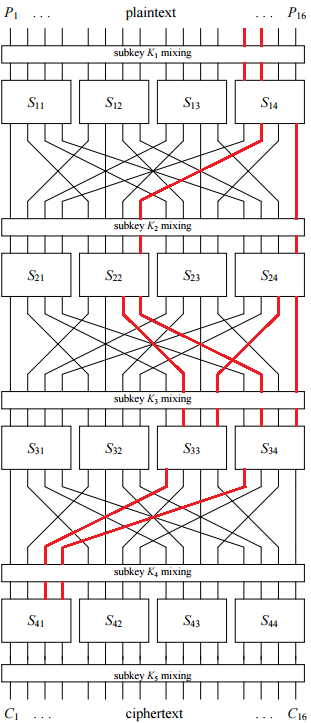
\includegraphics{12,12288}
  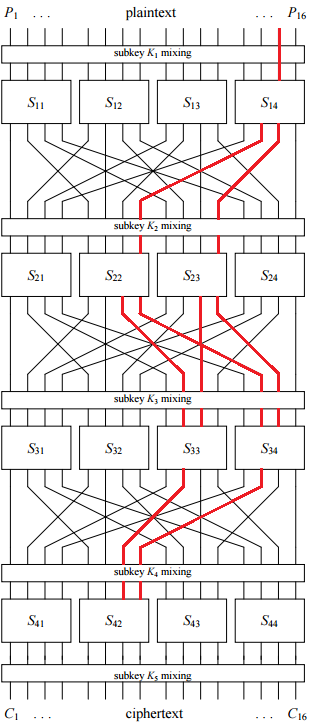
\includegraphics{13,768}

  \hspace{1cm}
  The diagrams above demonstrate the path through the substitution-permutation network undertaken to crack the first 8 bits of the subkey, using the differential pairs \lstinline{(12, 12288)} and \lstinline{(13, 768)} respectively.
  \clearpage
  
  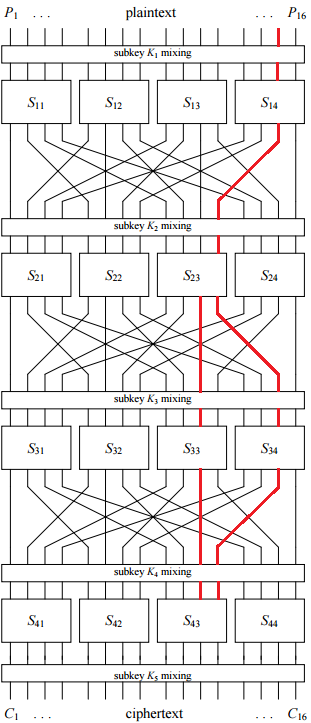
\includegraphics{2,48}
  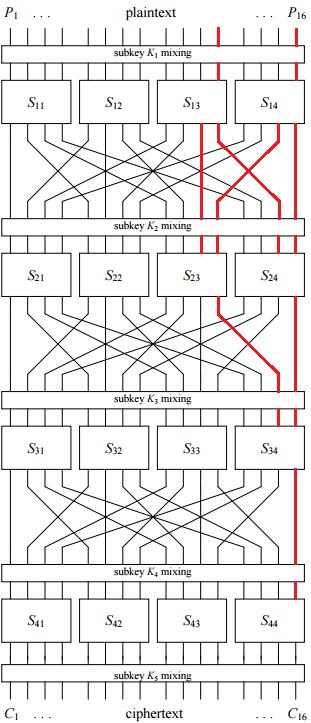
\includegraphics{17,1}

  \hspace{1cm}
  The diagrams above demonstrate the path through the substitution-permutation network undertaken to crack the last 8 bits of the subkey, using the differential pairs \lstinline{(2, 48)} and \lstinline{(17, 1)} respectively.
  \clearpage

\end{appendices}
\clearpage
\end{document}
